% do not edit the 4 lines below unless absolutely needed
\documentclass[twoside,twocolumn,10pt,a4paper]{IEEEtran}
\usepackage{graphics,epsfig,amsmath}
\usepackage{multirow,cite,hyperref}

% uncomment the following statement if Swedish is used
%\usepackage[swedish]{babel}


\begin{document}

\title{Title of Report in Biomedical Signal Processing}
\author{Name 1 (program-year, email address), Name 2 (program-year, email address)}
\maketitle


\begin{abstract}
The abstract should be 10--15 lines, and should mention the method(s), summarize the achieved results, and include a brief conclusion.
\end{abstract}

\section{Introduction}
Dialysis-induced hypotension continues to be a major complication in patients with end-stage renal disease undergoing hemodialysis, despite considerable effort to shed light on its underlying cause. Hypotension not only causes discomfort to the patient, but may increase mortality~\cite{Daugirdas1991}, \cite{Cavalcanti2004}. Since intradialytic hypotension leads to...

In this study, pulse oximetry is the starting point for developing a novel approach to the prediction of acute symptomatic, intradialytic hypotension. The method employs the normalized envelope of the PPG signal, measured at the finger, as an indirect measure of cardiac output and capillary vasoconstriction. The predictor is based on statistical detection theory, employing a model of the PPG signal in which the noise is assumed to be Laplacian. The different processing blocks that define the present method are displayed in Fig.~\ref{FigBlockDiagram}.

\begin{figure}[htbp]
\begin{center}
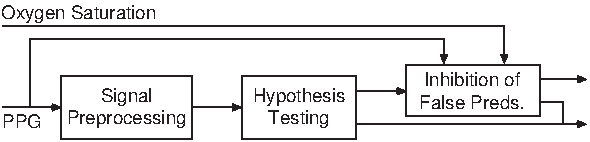
\includegraphics[scale=0.8]{BlockDiagram.pdf}
\caption{Block diagram of the method for prediction of acute symptomatic hypotension. The input signals are produced by a pulse oximeter. }
\label{FigBlockDiagram}
\end{center}
\end{figure}

%--------------------------------------------------------------------------------------------------------------------------------------------------
\section{Data}

%--------------------------------------------------------------------------------------------------------------------------------------------------
\section{Methods}

The PPG signal is first subjected to highpass filtering for the purpose of baseline wander removal as implemented by the following procedure. Since the acquisition device implements autoscaling (see below), low frequency information can be removed without causing problems. An estimate of the baseline wander is obtained by downsampling the PPG signal to $2$~Hz, followed by forward/backward filtering using a second order lowpass Butterworth filter with a cutoff frequency of $0.5$~Hz. The  lowpass filtered signal is then upsampled and subtracted from the original PPG signal, resulting in a highpass filtered signal denoted $p[k]$. It should be noted that the choice of cutoff frequency is not critical as subsequent signal processing does not rely on faithful pulse shape reproduction.

Changes in relative blood volume in the capillaries are assumed to be reflected by changes in the envelope of $p[k]$. A simple approach to obtaining a signal which reflects such changes is to compute the \textit{normalized integrated} PPG (niPPG) signal $x[n]$, defined by
\begin{equation}
x[n]= \frac{1}{\bar{P}} \sum_{k=nK-L+1}^{nK} \left | p[k] \right |,
\label{Part5_x[n]_from_p[k]}
\end{equation}
where $K$ and $L$ are positive integers that...

The detector structure is...

%--------------------------------------------------------------------------------------------------------------------------------------------------
\section{Results}
...


%--------------------------------------------------------------------------------------------------------------------------------------------------
\section{Discussion}
...


%--------------------------------------------------------------------------------------------------------------------------------------------------
\section{Conclusions}
...


%--------------------------------------------------------------------------------------------------------------------------------------------------
\begin{thebibliography}{10}

\bibitem{Daugirdas1991} J.T.~Daugirdas, ``Dialysis hypotension: a hemodynamic analysis,'' \emph{Kidney Int.}, vol.~39, pp.~233--246, 1991.

\bibitem{Cavalcanti2004} S.~Cavalcanti, A.~Ciandrini, S. Severi et al., ``Model-based study of the effects of the hemodialysis technique on the compensatory response to hypovolemia,'' \emph{Kidney Int.} vol.~65, pp.~1499--1510, 2004.

\bibitem{SornmoBioelectrical} L.~S{\"o}rnmo and P.~Laguna, {\em Bioelectrical Signal Processing in Cardiac and Neurological Applications}. Amsterdam: Elsevier (Academic Press), 2005.

\end{thebibliography}



\end{document}
 